\documentclass[border=10pt]{standalone}
\usepackage{pgfplots}
\pgfplotsset{compat=1.18}
\begin{document}
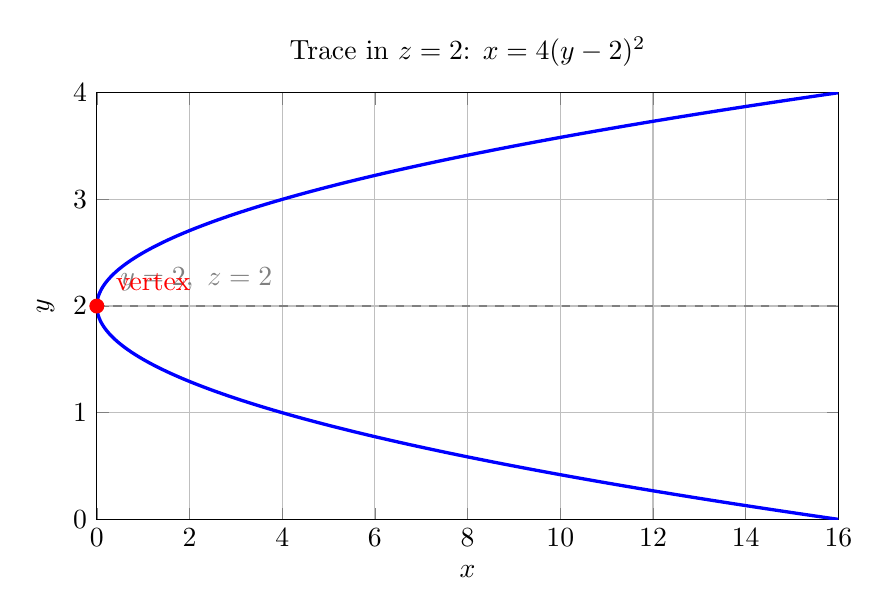
\begin{tikzpicture}
\begin{axis}[
    width=11cm,
    height=7cm,
    xlabel=$x$,
    ylabel=$y$,
    title={Trace in $z=2$: $x=4(y-2)^2$},
    domain=0:4,
    samples=200,
    grid=major,
    xmin=0, xmax=16,
    ymin=0, ymax=4,
]
\addplot[blue, very thick] ({4*(x-2)^2}, x);
\addplot[red, only marks, mark=*, mark size=2.5pt] coordinates {(0,2)};
\draw[gray, dashed] (axis cs:0,2) -- (axis cs:16,2);
\node[above right, gray] at (axis cs:0.3,2.05) {$y=2,\ z=2$};
\node[red, above right] at (axis cs:0.2,2.05) {vertex};
\end{axis}
\end{tikzpicture}
\end{document}